% Options for packages loaded elsewhere
\PassOptionsToPackage{unicode}{hyperref}
\PassOptionsToPackage{hyphens}{url}
%
\documentclass[
  man,floatsintext]{apa7}
\usepackage{amsmath,amssymb}
\usepackage{iftex}
\ifPDFTeX
  \usepackage[T1]{fontenc}
  \usepackage[utf8]{inputenc}
  \usepackage{textcomp} % provide euro and other symbols
\else % if luatex or xetex
  \usepackage{unicode-math} % this also loads fontspec
  \defaultfontfeatures{Scale=MatchLowercase}
  \defaultfontfeatures[\rmfamily]{Ligatures=TeX,Scale=1}
\fi
\usepackage{lmodern}
\ifPDFTeX\else
  % xetex/luatex font selection
\fi
% Use upquote if available, for straight quotes in verbatim environments
\IfFileExists{upquote.sty}{\usepackage{upquote}}{}
\IfFileExists{microtype.sty}{% use microtype if available
  \usepackage[]{microtype}
  \UseMicrotypeSet[protrusion]{basicmath} % disable protrusion for tt fonts
}{}
\makeatletter
\@ifundefined{KOMAClassName}{% if non-KOMA class
  \IfFileExists{parskip.sty}{%
    \usepackage{parskip}
  }{% else
    \setlength{\parindent}{0pt}
    \setlength{\parskip}{6pt plus 2pt minus 1pt}}
}{% if KOMA class
  \KOMAoptions{parskip=half}}
\makeatother
\usepackage{xcolor}
\usepackage{graphicx}
\makeatletter
\def\maxwidth{\ifdim\Gin@nat@width>\linewidth\linewidth\else\Gin@nat@width\fi}
\def\maxheight{\ifdim\Gin@nat@height>\textheight\textheight\else\Gin@nat@height\fi}
\makeatother
% Scale images if necessary, so that they will not overflow the page
% margins by default, and it is still possible to overwrite the defaults
% using explicit options in \includegraphics[width, height, ...]{}
\setkeys{Gin}{width=\maxwidth,height=\maxheight,keepaspectratio}
% Set default figure placement to htbp
\makeatletter
\def\fps@figure{htbp}
\makeatother
\setlength{\emergencystretch}{3em} % prevent overfull lines
\providecommand{\tightlist}{%
  \setlength{\itemsep}{0pt}\setlength{\parskip}{0pt}}
\setcounter{secnumdepth}{-\maxdimen} % remove section numbering
% Make \paragraph and \subparagraph free-standing
\ifx\paragraph\undefined\else
  \let\oldparagraph\paragraph
  \renewcommand{\paragraph}[1]{\oldparagraph{#1}\mbox{}}
\fi
\ifx\subparagraph\undefined\else
  \let\oldsubparagraph\subparagraph
  \renewcommand{\subparagraph}[1]{\oldsubparagraph{#1}\mbox{}}
\fi
\newlength{\cslhangindent}
\setlength{\cslhangindent}{1.5em}
\newlength{\csllabelwidth}
\setlength{\csllabelwidth}{3em}
\newlength{\cslentryspacingunit} % times entry-spacing
\setlength{\cslentryspacingunit}{\parskip}
\newenvironment{CSLReferences}[2] % #1 hanging-ident, #2 entry spacing
 {% don't indent paragraphs
  \setlength{\parindent}{0pt}
  % turn on hanging indent if param 1 is 1
  \ifodd #1
  \let\oldpar\par
  \def\par{\hangindent=\cslhangindent\oldpar}
  \fi
  % set entry spacing
  \setlength{\parskip}{#2\cslentryspacingunit}
 }%
 {}
\usepackage{calc}
\newcommand{\CSLBlock}[1]{#1\hfill\break}
\newcommand{\CSLLeftMargin}[1]{\parbox[t]{\csllabelwidth}{#1}}
\newcommand{\CSLRightInline}[1]{\parbox[t]{\linewidth - \csllabelwidth}{#1}\break}
\newcommand{\CSLIndent}[1]{\hspace{\cslhangindent}#1}
\ifLuaTeX
\usepackage[bidi=basic]{babel}
\else
\usepackage[bidi=default]{babel}
\fi
\babelprovide[main,import]{english}
% get rid of language-specific shorthands (see #6817):
\let\LanguageShortHands\languageshorthands
\def\languageshorthands#1{}
% Manuscript styling
\usepackage{upgreek}
\captionsetup{font=singlespacing,justification=justified}

% Table formatting
\usepackage{longtable}
\usepackage{lscape}
% \usepackage[counterclockwise]{rotating}   % Landscape page setup for large tables
\usepackage{multirow}		% Table styling
\usepackage{tabularx}		% Control Column width
\usepackage[flushleft]{threeparttable}	% Allows for three part tables with a specified notes section
\usepackage{threeparttablex}            % Lets threeparttable work with longtable

% Create new environments so endfloat can handle them
% \newenvironment{ltable}
%   {\begin{landscape}\centering\begin{threeparttable}}
%   {\end{threeparttable}\end{landscape}}
\newenvironment{lltable}{\begin{landscape}\centering\begin{ThreePartTable}}{\end{ThreePartTable}\end{landscape}}

% Enables adjusting longtable caption width to table width
% Solution found at http://golatex.de/longtable-mit-caption-so-breit-wie-die-tabelle-t15767.html
\makeatletter
\newcommand\LastLTentrywidth{1em}
\newlength\longtablewidth
\setlength{\longtablewidth}{1in}
\newcommand{\getlongtablewidth}{\begingroup \ifcsname LT@\roman{LT@tables}\endcsname \global\longtablewidth=0pt \renewcommand{\LT@entry}[2]{\global\advance\longtablewidth by ##2\relax\gdef\LastLTentrywidth{##2}}\@nameuse{LT@\roman{LT@tables}} \fi \endgroup}

% \setlength{\parindent}{0.5in}
% \setlength{\parskip}{0pt plus 0pt minus 0pt}

% Overwrite redefinition of paragraph and subparagraph by the default LaTeX template
% See https://github.com/crsh/papaja/issues/292
\makeatletter
\renewcommand{\paragraph}{\@startsection{paragraph}{4}{\parindent}%
  {0\baselineskip \@plus 0.2ex \@minus 0.2ex}%
  {-1em}%
  {\normalfont\normalsize\bfseries\itshape\typesectitle}}

\renewcommand{\subparagraph}[1]{\@startsection{subparagraph}{5}{1em}%
  {0\baselineskip \@plus 0.2ex \@minus 0.2ex}%
  {-\z@\relax}%
  {\normalfont\normalsize\itshape\hspace{\parindent}{#1}\textit{\addperi}}{\relax}}
\makeatother

% \usepackage{etoolbox}
\makeatletter
\patchcmd{\HyOrg@maketitle}
  {\section{\normalfont\normalsize\abstractname}}
  {\section*{\normalfont\normalsize\abstractname}}
  {}{\typeout{Failed to patch abstract.}}
\patchcmd{\HyOrg@maketitle}
  {\section{\protect\normalfont{\@title}}}
  {\section*{\protect\normalfont{\@title}}}
  {}{\typeout{Failed to patch title.}}
\makeatother

\usepackage{xpatch}
\makeatletter
\xapptocmd\appendix
  {\xapptocmd\section
    {\addcontentsline{toc}{section}{\appendixname\ifoneappendix\else~\theappendix\fi\\: #1}}
    {}{\InnerPatchFailed}%
  }
{}{\PatchFailed}
\keywords{keywords\newline\indent Word count: X}
\usepackage{lineno}

\linenumbers
\usepackage{csquotes}
\makeatletter
\renewcommand{\paragraph}{\@startsection{paragraph}{4}{\parindent}%
  {0\baselineskip \@plus 0.2ex \@minus 0.2ex}%
  {-1em}%
  {\normalfont\normalsize\bfseries\typesectitle}}

\renewcommand{\subparagraph}[1]{\@startsection{subparagraph}{5}{1em}%
  {0\baselineskip \@plus 0.2ex \@minus 0.2ex}%
  {-\z@\relax}%
  {\normalfont\normalsize\bfseries\itshape\hspace{\parindent}{#1}\textit{\addperi}}{\relax}}
\makeatother

\ifLuaTeX
  \usepackage{selnolig}  % disable illegal ligatures
\fi
\IfFileExists{bookmark.sty}{\usepackage{bookmark}}{\usepackage{hyperref}}
\IfFileExists{xurl.sty}{\usepackage{xurl}}{} % add URL line breaks if available
\urlstyle{same}
\hypersetup{
  pdftitle={Psychopathy, borderline personality disorder, and emotional processing in incarcerated women},
  pdfauthor={Annalise S Halverson1 \& Natalie Dowling1,2},
  pdflang={en-EN},
  pdfkeywords={keywords},
  hidelinks,
  pdfcreator={LaTeX via pandoc}}

\title{Psychopathy, borderline personality disorder, and emotional processing in incarcerated women}
\author{Annalise S Halverson\textsuperscript{1} \& Natalie Dowling\textsuperscript{1,2}}
\date{}


\shorttitle{psychopathy and psychopathology correlates in women}

\authornote{

Add complete departmental affiliations for each author here. Each new line herein must be indented, like this line.

Enter author note here.

The authors made the following contributions. Annalise S Halverson: Conceptualization, Writing - Original Draft Preparation, Writing - Review \& Editing; Natalie Dowling: Writing - Review \& Editing, Supervision.

Correspondence concerning this article should be addressed to Annalise S Halverson, 5848 S University Ave, Chicago, IL, 60637. E-mail: \href{mailto:asdh@uchicago.edu}{\nolinkurl{asdh@uchicago.edu}}

}

\affiliation{\vspace{0.5cm}\textsuperscript{1} University of Chicago\\\textsuperscript{2} Department of Psychology}

\abstract{%
One or two sentences providing a \textbf{basic introduction} to the field, comprehensible to a scientist in any discipline.
Two to three sentences of \textbf{more detailed background}, comprehensible to scientists in related disciplines.
One sentence clearly stating the \textbf{general problem} being addressed by this particular study.
One sentence summarizing the main result (with the words ``\textbf{here we show}'' or their equivalent).
Two or three sentences explaining what the \textbf{main result} reveals in direct comparison to what was thought to be the case previously, or how the main result adds to previous knowledge.
One or two sentences to put the results into a more \textbf{general context}.
Two or three sentences to provide a \textbf{broader perspective}, readily comprehensible to a scientist in any discipline.
}



\begin{document}
\maketitle

\hypertarget{introduction}{%
\section{Introduction}\label{introduction}}

Psychopathy as a construct has undergone detailed iterations to annotate its numerous idiosyncrasies. Around 1.2\% of American men and 0.5\% of American women are believed to possess clinically significant levels of psychopathic traits (Barbara Burton \& Fabian M. Saleh, 2020). While persistent antisocial conduct is commonly present, psychopathy is also uniquely characterized by absences -- notably a deficiency in emotional reaction and a lack of empathy or remorse (De Brito et al., 2021; Sellbom \& Drislane, 2021). It spans race, gender, socioeconomic status, and culture, and further possesses a kaleidoscope of consequences -- from disturbed well-being to increased involvement in the criminal justice system. While it is believed to be present in around 1\% of the general population, an estimated 15-25\% of those incarcerated are likely to fall somewhere on the psychopathy spectrum (Barbara Burton \& Fabian M. Saleh, 2020).

A discrimination in subtypes of psychopathy was pioneered by Karpman (1941), who proposed the existence of two groups: primary and secondary. Primary psychopaths are exceedingly low in anxiety and predisposed to be antisocial, whereas secondary psychopaths become callous and high in anxiety as a response to various vulnerabilities in the environment (Sellbom \& Drislane, 2021). The most widely investigated measure of psychopathy to-date originates in Cleckley's (1976) conception of psychopathy. The framework is divided into interpersonal-affective -- or Factor 1 -- traits and lifestyle-antisocial -- or Factor 2 -- traits. Factor 1 traits include superficial charm, a grandiose sense of self-worth, and lack of empathy or remorse; Factor 2 traits are characterized by early behavioral problems and delinquency, as well as impulsivity and a proneness to boredom (De Brito et al., 2021). These factors are distinct (Hunt et al., 2015) but not mutually exclusive; persons demonstrating high interactions of Factor 1 and Factor 2 traits are considered high in psychopathic tendencies, and diluted exhibitions in one or the other consequentially fall lower on the spectrum (Verona et al., 2012). The Psychopathy Checklist---Revised (PCL---R; Hare, 2003) borne from this composition, and it is the chief measure of psychopathy that will be utilized in the present study.

Discrepancies in our understanding of psychopathy as it pertains to women sparked interest in this discourse, namely a murky association with previously correlated externalizing disorders -- such as antisocial personality disorder and narcissistic personality disorder (De Vogel \& Lancel, 2016; Rutherford et al., 1998) -- and the tendency for women to score lower than men across rating scales (Newhill et al., 2010; Spormann et al., 2023). While Cleckley's criteria, are often considered immune to gender stereotypes, these divergences highlighted the possibility that researchers were examining the wrong traits, or perhaps searching for misrepresentative correlates (Vitale \& Newman, 2001).

Recent studies examining gender differences have found women with psychopathy to possess less overall deficits in emotional processing, as well as show less physical violence while exhibiting heightened manipulative and self-destructive behaviors, possibly from learning how to compensate through socialization (for a review, see Efferson \& Glenn, 2018); they are also more often diagnosed with borderline personality disorder compared to men with psychopathy (De Vogel \& Lancel, 2016). Borderline personality disorder (BPD) is characterized by unstable and explosive emotional patterns. Those diagnosed with BPD often struggle to both maintain relationships and inhibit chaotic impulses (Clarkin \& Posner, 2005). It is estimated that 1.4\% of the adult U.S. population is eligible for BPD diagnosis; nearly 75\% of those diagnosed are women (National Institute of Mental Health, 2023). Zlotnick et al. (2002) found BPD-diagnosed women were more likely than BPD-diagnosed men to meet criteria for internalizing and impulse-defined comorbidities -- such as eating disorder, panic disorder, and major depressive disorder. These correlations paint an image of high levels of inner distress in the wake of negative affect for women with BPD, which may have interesting connotations for how it relates to coexisting conditions that also impact emotional regulation, such as psychopathy.

Alexithymia is a syndrome marked by hindrances in experiencing, identifying, and expressing emotions. Like psychopathy, the construct is multifaceted and possesses both cognitive and affective components (Goerlich, 2018). Decreased emotional awareness may thwart social development, making alexithymia highly pertinent to both daily functioning and the onset of psychiatric disorders. As traits of both psychopathy and BPD evidently alter emotional regulation and processing, it is likely associations would be found between its diagnosis and the presence of alexithymia. Ridings and Lutz-Zois (2014) suggested BPD may act as a mediator in the association between secondary psychopathy and alexithymia. A 2022 meta-analysis by Burghart and Mier elicited positive associations between psychopathy and alexithymia, as well its sub-components -- difficulty describing feelings, difficulty identifying feelings, and externally-oriented thinking. Examining gender as a moderator, they found the association between psychopathy and overall alexithymia to be stronger in women compared to men.

It is unclear how thoroughly these findings might translate onto clinical or special populations. Special populations are useful for research as they can provide valuable insight along the margins of spectra that may be overlooked. We now stand at an intersection of extremities, as this study aims to clarify how the interaction between psychopathy and borderline personality disorder may impact one's ability to experience, identify, or express emotions when impairments are more clinically severe.

\hypertarget{present-aims}{%
\section{Present Aims}\label{present-aims}}

Stimulating research continues to emerge regarding the relationship between psychopathy and BPD, as well as emotional dysregulation and BPD. However, the impact BPD and psychopathy may have on women with respect to their ability to experience, identify, or express emotions is at present underexplored. Further, special populations are often underrepresented in research and thus critical to mapping out the spectrum of impact. A primary aim of the present study is to delineate the clinical presentation of psychopathy in incarcerated women as it intersects with borderline personality disorder and alexithymia. Poor empathy and emotional dysregulation render psychopathy a prevalent risk factor for severe and chronic violence. While criminality is not a certainty, understanding how the condition hardens along this lineage could have meaningful benefits in the clinical sphere and thus guide necessary treatment to lower both violent onset and recidivism rates. Treatment is especially pertinent for those in vulnerable populations who may be limited in access.

Contrary to male psychopathy, female psychopathy has been shown to possess a much stronger association with tendencies of borderline personality disorder (Sprague et al., 2012). It is hypothesized that borderline personality disorder will mediate the relationship between psychopathy and alexithymia (see below graphic, no clue how to reference right now). The literature has made abundantly clear the manifold expressions of psychopathy; as such, it is important this diversity is accounted for in our research. Results are likely to have implications for both forensic practice and neuroscientific theory.

\begin{figure}
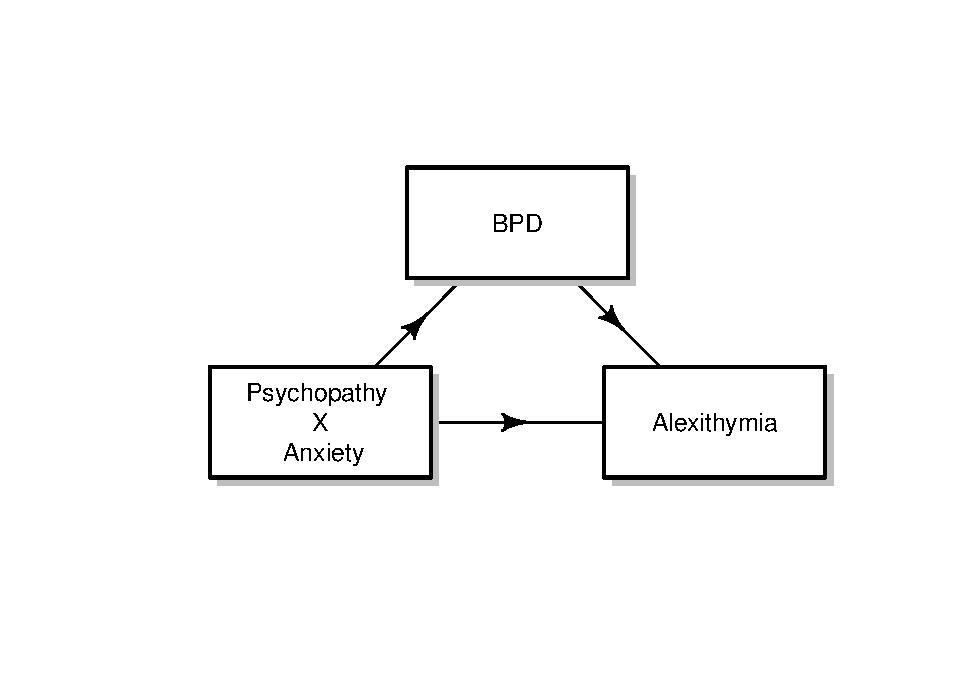
\includegraphics[width=1\linewidth]{d2m-Psychopathy_files/figure-latex/simple plot of mediation relationship-1} \caption{ }(\#fig:simple plot of mediation relationship)
\end{figure}

\hypertarget{methods}{%
\section{Methods}\label{methods}}

We report how we determined our sample size, all data exclusions (if any), all manipulations, and all measures in the study.

\hypertarget{participants}{%
\subsection{Participants}\label{participants}}

\hypertarget{measures}{%
\subsection{Measures}\label{measures}}

\begin{itemize}
\tightlist
\item
  make sure to note here why interaction
\end{itemize}

\hypertarget{procedure}{%
\subsection{Procedure}\label{procedure}}

Of the 156 total participants, 52 participants failed to complete one or more of the four assessments. Due to the nature of the variables, it was determined most ethical to simply remove participants who were missing data for any of the required assessments. A total of 104 participants remained for further analysis.

\hypertarget{data-analysis}{%
\subsection{Data analysis}\label{data-analysis}}

We used R (Version 4.3.2; R Core Team, 2023) and the R-packages \emph{diagram} (Version 1.6.5; Soetaert, 2020), \emph{dplyr} (Version 1.1.4; Wickham, François, et al., 2023), \emph{forcats} (Version 1.0.0; Wickham, 2023a), \emph{ggformula} (Version 0.12.0; Kaplan \& Pruim, 2023), \emph{ggplot2} (Version 3.4.4; Wickham, 2016), \emph{ggsci} (Version 3.0.0; Xiao, 2023), \emph{kableExtra} (Version 1.4.0; Zhu, 2024), \emph{lattice} (Version 0.21.9; Sarkar, 2008), \emph{lubridate} (Version 1.9.3; Grolemund \& Wickham, 2011), \emph{MASS} (Version 7.3.60; Venables \& Ripley, 2002), \emph{Matrix} (Version 1.6.1.1; Bates et al., 2023), \emph{mediation} (Imai, Keele, \& Yamamoto, 2010; Imai, Keele, \& Tingley, 2010; Imai et al., 2011; Imai \& Yamamoto, 2013; Version 4.5.0; Tingley et al., 2014), \emph{mosaic} (Version 1.9.0; Pruim et al., 2017, 2023), \emph{mosaicData} (Version 0.20.4; Pruim et al., 2023), \emph{mvtnorm} (Version 1.2.4; Genz \& Bretz, 2009), \emph{papaja} (Version 0.1.1.9001; Aust \& Barth, 2023), \emph{plot.matrix} (Version 1.6.2; Klinke, 2022), \emph{psych} (Version 2.4.1; William Revelle, 2024), \emph{purrr} (Version 1.0.2; Wickham \& Henry, 2023), \emph{readr} (Version 2.1.4; Wickham, Hester, et al., 2023), \emph{readxl} (Version 1.4.3; Wickham \& Bryan, 2023), \emph{sandwich} (Zeileis, 2004, 2006; Version 3.1.0; Zeileis et al., 2020), \emph{shape} (Version 1.4.6; Soetaert, 2021), \emph{stargazer} (Version 5.2.3; Hlavac, 2022), \emph{stringr} (Version 1.5.1; Wickham, 2023b), \emph{tibble} (Version 3.2.1; Müller \& Wickham, 2023), \emph{tidyr} (Version 1.3.1; Wickham, Vaughan, et al., 2023), \emph{tidyverse} (Version 2.0.0; Wickham et al., 2019), and \emph{tinylabels} (Version 0.2.4; Barth, 2023) for all our analyses.

\hypertarget{results}{%
\section{Results}\label{results}}

\begin{table}[!htbp] \centering 
  \caption{Summary Table} 
  \label{tab:summary-table} 
\begin{tabular}{@{\extracolsep{5pt}}lccccc} 
\\[-1.8ex]\hline 
\hline \\[-1.8ex] 
Statistic & \multicolumn{1}{c}{N} & \multicolumn{1}{c}{Mean} & \multicolumn{1}{c}{St. Dev.} & \multicolumn{1}{c}{Min} & \multicolumn{1}{c}{Max} \\ 
\hline \\[-1.8ex] 
PAIBOR\_Total\_Score & 104 & 36.750 & 11.738 & 11 & 58 \\ 
PCLR\_Total\_Score\_Prorated & 104 & 23.476 & 8.070 & 4.400 & 37.000 \\ 
TAS\_Total\_Score & 104 & 49.702 & 13.852 & 20 & 82 \\ 
STAI\_Trait\_Anxiety & 104 & 45.558 & 11.213 & 23 & 72 \\ 
\hline \\[-1.8ex] 
\end{tabular} 
\end{table}

Descriptive statistics for the assessments of interest can be seen in Table~\ref{tab:summary-table}.



\begin{verbatim}
## Warning: Removed 2 rows containing missing values (`geom_bar()`).
\end{verbatim}

\begin{figure}
\centering
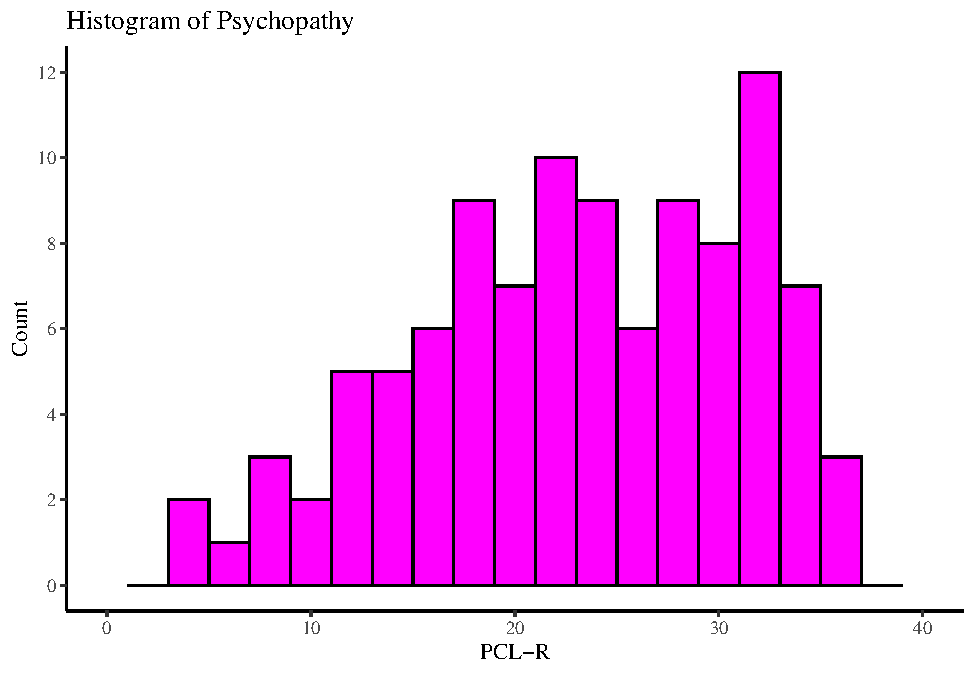
\includegraphics{d2m-Psychopathy_files/figure-latex/PCLR-descriptives-1.pdf}
\caption{\label{fig:PCLR-descriptives}Histogram of score distribution on the PCL--R.}
\end{figure}

As seen in Figure~\ref{fig:PCLR-descriptives}, our distribution of PCL--R scores is left-skewed, with more participants falling on the higher end of the spectrum. This is ?consistent? with past studies conducted with incarcerated populations (probably Decety). Other score assessment distributions can be found in the appendix.

\begin{verbatim}
## Warning: Removed 2 rows containing missing values (`geom_bar()`).
\end{verbatim}

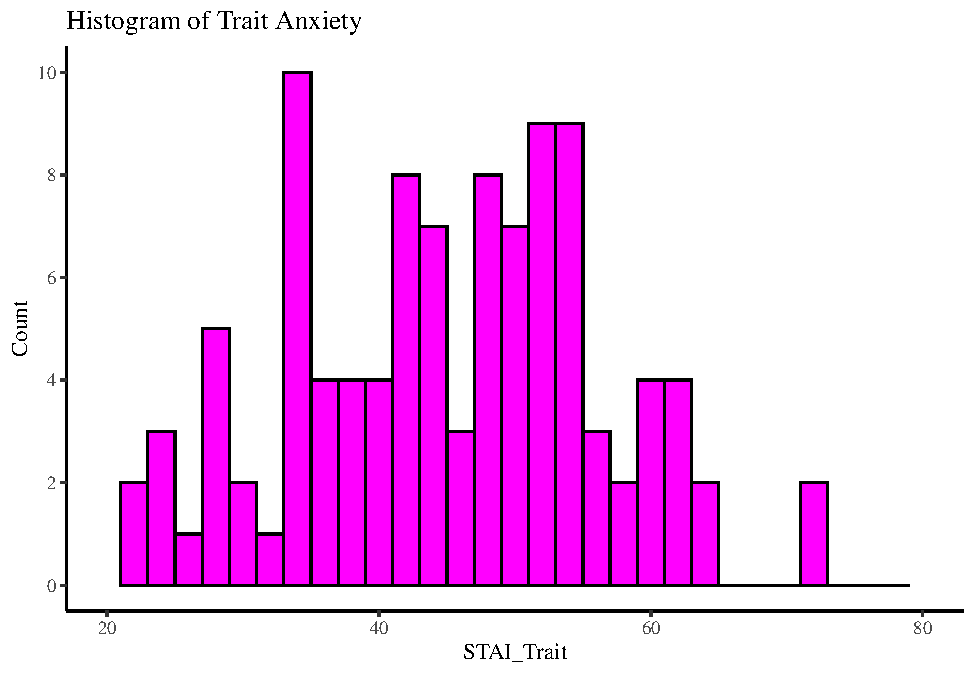
\includegraphics{d2m-Psychopathy_files/figure-latex/STAI-descriptives-1.pdf}

\begin{verbatim}
## Warning: Removed 1 rows containing missing values (`geom_bar()`).
\end{verbatim}

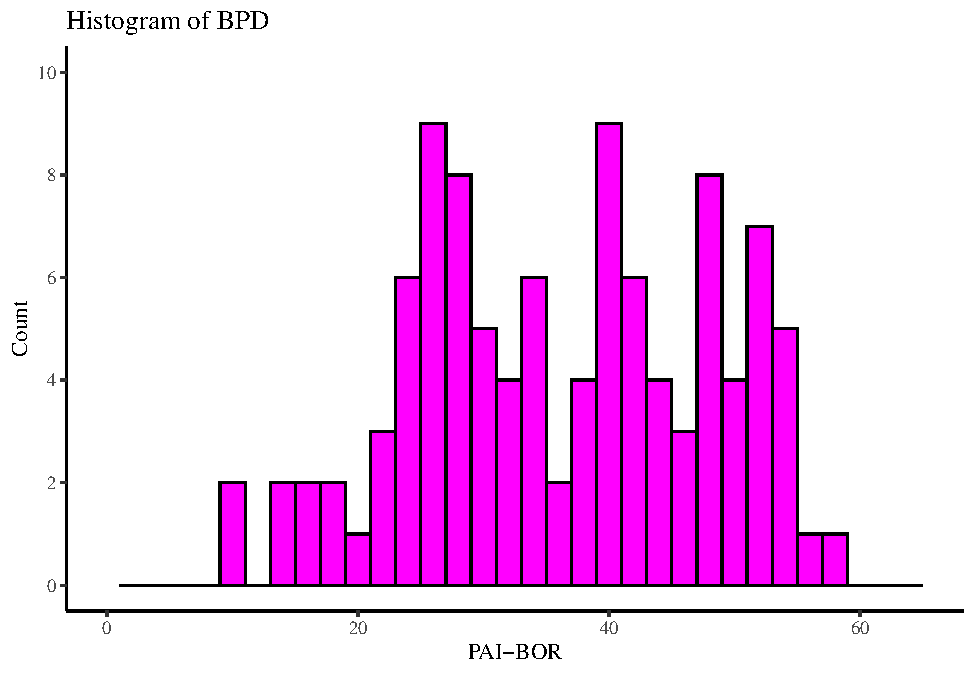
\includegraphics{d2m-Psychopathy_files/figure-latex/PAI-descriptives-1.pdf}

\begin{verbatim}
## Warning: Removed 1 rows containing non-finite values (`stat_bin()`).
\end{verbatim}

\begin{verbatim}
## Warning: Removed 2 rows containing missing values (`geom_bar()`).
\end{verbatim}

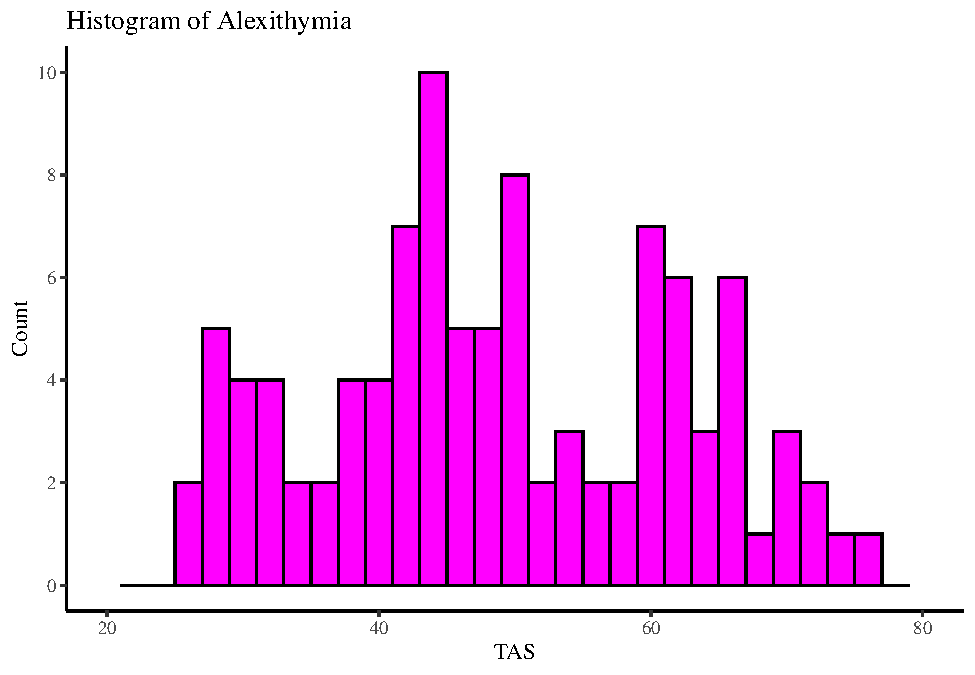
\includegraphics{d2m-Psychopathy_files/figure-latex/TAS-descriptives-1.pdf}

The mean PCL--R score is 23.48.

The mean PAI--BOR score is 36.75.

The mean TAS score is 49.70.



\begin{figure}
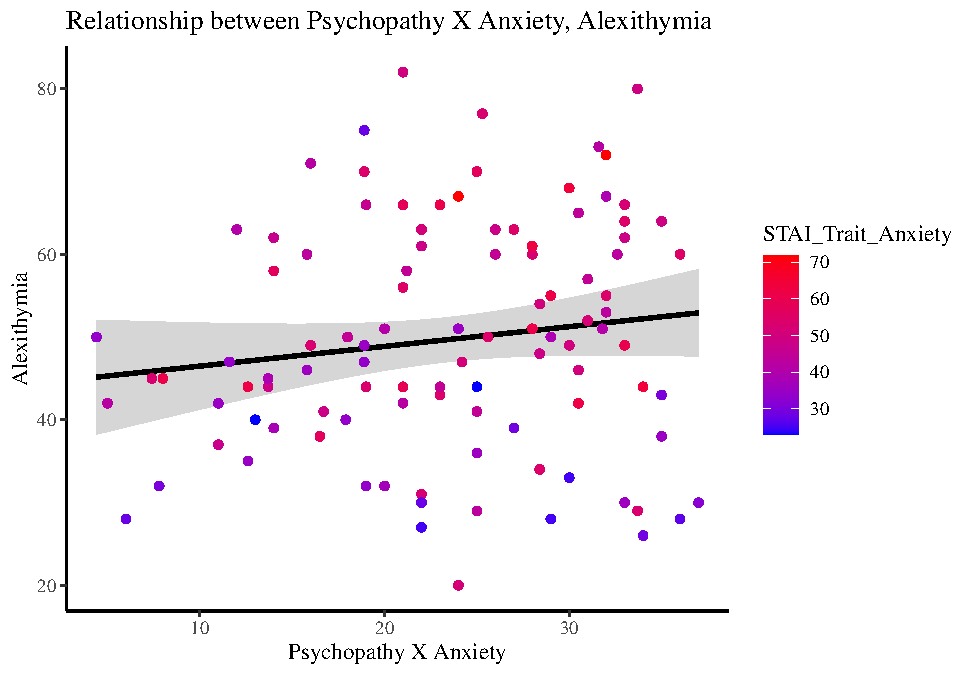
\includegraphics[width=1\linewidth]{d2m-Psychopathy_files/figure-latex/c-path-scatterplot-1} \caption{Scatterplot demonstrating relationship between the interactive term of psychopathy and trait anxiety with alexithymia in our sample of incarcerated women.}\label{fig:c-path-scatterplot}
\end{figure}

Figure~\ref{fig:c-path-scatterplot} shows a moderate correlation of 0.37 between PsychopathyXAnxiety and Alexithymia. \ldots{}



\begin{figure}
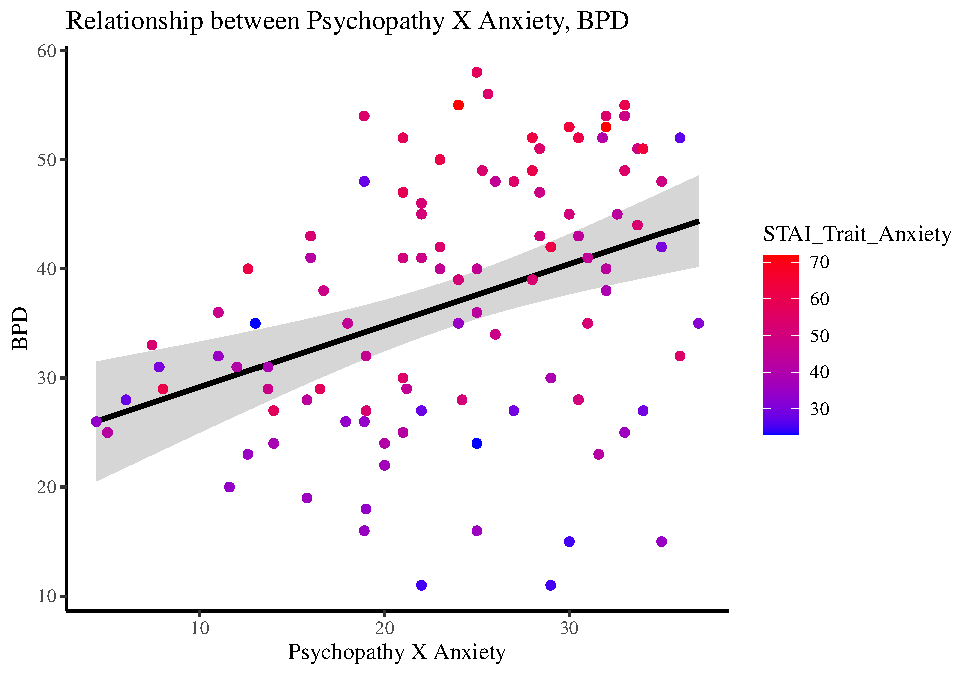
\includegraphics[width=1\linewidth]{d2m-Psychopathy_files/figure-latex/a-path-scatterplot-1} \caption{Scatterplot demonstrating relationship between the interactive term of psychopathy and trait anxiety with borderline personality disorder in our sample of incarcerated women.}\label{fig:a-path-scatterplot}
\end{figure}

Figure~\ref{fig:a-path-scatterplot} shows a moderate to strong correlation of 0.66 between PsychopathyXAnxiety and BPD. \ldots{}

All assessment scores (including the interactive term) were standardized. Mediation analyses with bootstrapping were conducted to test the primary hypothesis. Unlike other methods, bootstrapping is not limited by the assumption of normality. The interaction term of PCL--R Total Score and STAI Trait Anxiety was entered as the predictor, and PAI-BOR Total Score was entered as the mediating term. Total Score on the TAS was our outcome variable. A significant Average Causal Mediation Effect (ACME) would demonstrate support of our hypothesis. Summary tables (figure out how to include this info) show that the ACME is significant and the Average Direct Effect (ADE) disappears. This implies full causal mediation by BPD on the relationship between PsychopathyXAnxiety and Alexithymia.

\begin{table}[!htbp] \centering 
  \caption{Preliminary Regression Results} 
  \label{tab:prelim-regression-output} 
\begin{tabular}{@{\extracolsep{1pt}}lccc} 
\\[-1.8ex]\hline 
\hline \\[-1.8ex] 
 & \multicolumn{3}{c}{\textit{Dependent variable:}} \\ 
\cline{2-4} 
\\[-1.8ex] & P-O Path & P-M Path & M-O Path \\ 
\\[-1.8ex] & (1) & (2) & (3)\\ 
\hline \\[-1.8ex] 
 PsychopathyXAnxiety & 0.373$^{***}$ & 0.660$^{***}$ &  \\ 
  & (0.092) & (0.074) &  \\ 
  & & & \\ 
 BPD &  &  & 0.471$^{***}$ \\ 
  &  &  & (0.087) \\ 
  & & & \\ 
 Constant & $-$0.000 & $-$0.000 & $-$0.000 \\ 
  & (0.091) & (0.074) & (0.087) \\ 
  & & & \\ 
\hline \\[-1.8ex] 
Observations & 104 & 104 & 104 \\ 
R$^{2}$ & 0.139 & 0.436 & 0.222 \\ 
Adjusted R$^{2}$ & 0.131 & 0.431 & 0.214 \\ 
Residual Std. Error (df = 102) & 0.932 & 0.755 & 0.887 \\ 
F Statistic (df = 1; 102) & 16.501$^{***}$ & 78.905$^{***}$ & 29.024$^{***}$ \\ 
\hline 
\hline \\[-1.8ex] 
\textit{Note:}  & \multicolumn{3}{r}{$^{*}$p$<$0.1; $^{**}$p$<$0.05; $^{***}$p$<$0.01} \\ 
\end{tabular} 
\end{table}

In order to run a mediation analysis, one must ensure significant relationships exist between predictor and outcome, predictor and mediator, and mediator and outcome. Results for these preliminary analyses can be seen in Table~\ref{tab:prelim-regression-output}.

\begin{table}[!htbp] \centering 
  \caption{Simple Linear Regression Results} 
  \label{tab:simple-regression-output} 
\begin{tabular}{@{\extracolsep{1pt}}lcccc} 
\\[-1.8ex]\hline 
\hline \\[-1.8ex] 
 & \multicolumn{4}{c}{\textit{Dependent variable:}} \\ 
\cline{2-5} 
\\[-1.8ex] & TAS Total & Factor 1 & Factor 2 & Factor 3 \\ 
\\[-1.8ex] & (1) & (2) & (3) & (4)\\ 
\hline \\[-1.8ex] 
 PsychopathyXAnxiety & 0.373$^{***}$ & 0.418$^{***}$ & 0.291$^{***}$ & 0.197$^{**}$ \\ 
  & (0.092) & (0.090) & (0.095) & (0.097) \\ 
  & & & & \\ 
 Constant & $-$0.000 & $-$0.000 & $-$0.000 & 0.000 \\ 
  & (0.091) & (0.090) & (0.094) & (0.097) \\ 
  & & & & \\ 
\hline \\[-1.8ex] 
Observations & 104 & 104 & 104 & 104 \\ 
R$^{2}$ & 0.139 & 0.174 & 0.085 & 0.039 \\ 
Adjusted R$^{2}$ & 0.131 & 0.166 & 0.076 & 0.030 \\ 
Residual Std. Error (df = 102) & 0.932 & 0.913 & 0.961 & 0.985 \\ 
F Statistic (df = 1; 102) & 16.501$^{***}$ & 21.551$^{***}$ & 9.463$^{***}$ & 4.140$^{**}$ \\ 
\hline 
\hline \\[-1.8ex] 
\textit{Note:}  & \multicolumn{4}{r}{$^{*}$p$<$0.1; $^{**}$p$<$0.05; $^{***}$p$<$0.01} \\ 
\end{tabular} 
\end{table}

\begin{table}[!htbp] \centering 
  \caption{Multiple Linear Regression Results} 
  \label{tab:mult-regression-output} 
\begin{tabular}{@{\extracolsep{1pt}}lcccc} 
\\[-1.8ex]\hline 
\hline \\[-1.8ex] 
 & \multicolumn{4}{c}{\textit{Dependent variable:}} \\ 
\cline{2-5} 
\\[-1.8ex] & TAS Total & Factor 1 & Factor 2 & Factor 3 \\ 
\\[-1.8ex] & (1) & (2) & (3) & (4)\\ 
\hline \\[-1.8ex] 
 PsychopathyXAnxiety & 0.111 & 0.096 & 0.036 & 0.154 \\ 
  & (0.116) & (0.110) & (0.121) & (0.130) \\ 
  & & & & \\ 
 BPD & 0.398$^{***}$ & 0.487$^{***}$ & 0.386$^{***}$ & 0.066 \\ 
  & (0.116) & (0.110) & (0.121) & (0.130) \\ 
  & & & & \\ 
 Constant & $-$0.000 & $-$0.000 & $-$0.000 & 0.000 \\ 
  & (0.087) & (0.082) & (0.090) & (0.097) \\ 
  & & & & \\ 
\hline \\[-1.8ex] 
Observations & 104 & 104 & 104 & 104 \\ 
R$^{2}$ & 0.228 & 0.308 & 0.169 & 0.041 \\ 
Adjusted R$^{2}$ & 0.213 & 0.294 & 0.153 & 0.022 \\ 
Residual Std. Error (df = 101) & 0.887 & 0.840 & 0.921 & 0.989 \\ 
F Statistic (df = 2; 101) & 14.949$^{***}$ & 22.477$^{***}$ & 10.273$^{***}$ & 2.182 \\ 
\hline 
\hline \\[-1.8ex] 
\textit{Note:}  & \multicolumn{4}{r}{$^{*}$p$<$0.1; $^{**}$p$<$0.05; $^{***}$p$<$0.01} \\ 
\end{tabular} 
\end{table}

There is a significant relationship between predictor and outcome (\emph{p} = ). However, this effect goes away when adding BPD as a mediator (\emph{p} = ). This suggests that the presence of BPD acts as a mechanism through which the predictor influences the outcome. The significant, full mediation effect we observed suggests that a portion of the total effect of the predictor on the outcome is explained by the mediator (\emph{p} = ).

Three subfactors defined in the TAS are believed to compose alexithymia: difficulty identifying feelings (Factor 1), difficulty describing feelings (Factor 2), and externally-oriented thinking (Factor 3). As we collected subfactor scores for every participant, an exploratory analysis could be conducted to get a sense of what specific parts of emotional processing psychopathy and BPD may be impacting. We found that, replacing the total TAS score for Factor 1 and Factor 2, the significant mediation effect remained in tact. However, designating Factor 3 as an outcome left us with an insignificant model. The change in significant effect when replacing for specific factors of TAS suggests the mediation effect may depend on specific aspects or dimensions of alexithymia. It is critical these results are analyzed with caution as no hypotheses regarding TAS subfactors were determined a priori and the theoretical lineage is at present quite limited.

\hypertarget{discussion}{%
\section{Discussion}\label{discussion}}

It is possible that BPD symptoms uniquely impact certain dimensions of the outcome variable. When considering what each of the three factors represent, it may be plausible that BPD would affect factors 1 and 2 -- addressing emotional comprehension and recognition -- and not 3, as BPD may be more closely associated with internalizing features. More research that addresses the role of BPD on externally-oriented thinking is required here to draw firmer conclusions.

It is without a doubt that the relationship between psychopathy, anxiety, BPD, and alexithymia is multifaceted and complex. Our results should be further interpreted with caution and a unique sample such as this one may lead to skewed distributions.

Additional factors and moderators warrant further exploration. Other relevant comorbidities -- such as PTSD -- may influence the heterogeneous mediation pathway seen here in a way that could explain the nuanced relationships further. Further, it would certainly be worthwhile to break down BPD further to understand what specific mechanisms of this disorder might be at play in this relationship. We did not have sufficient data to conduct a factor analysis, but it may be useful as the personality disorder can be diagnosed in 256 unique ways, according to the DSM-V.

The heterogeneity of this mediation effect is certainly cause for future research. This information can guide the development of targeted interventions or strategies based on specific factors that are most influenced by the mediation process. This changes in significance emphasize the need for careful and nuanced interpretation, taking into account the specific characteristics and dynamics at play for each factor within the composite variables.

\newpage

\hypertarget{references}{%
\section{References}\label{references}}

\hypertarget{refs}{}
\begin{CSLReferences}{1}{0}
\leavevmode\vadjust pre{\hypertarget{ref-R-papaja}{}}%
Aust, F., \& Barth, M. (2023). \emph{{papaja}: {Prepare} reproducible {APA} journal articles with {R Markdown}}. \url{https://github.com/crsh/papaja}

\leavevmode\vadjust pre{\hypertarget{ref-barbaraburtonPsychopathyInsightsGeneral2020}{}}%
Barbara Burton, M. D., \& Fabian M. Saleh, M. D. (2020). \emph{Psychopathy: {Insights} for {General Practice}}. \emph{37}.

\leavevmode\vadjust pre{\hypertarget{ref-R-tinylabels}{}}%
Barth, M. (2023). \emph{{tinylabels}: Lightweight variable labels}. \url{https://cran.r-project.org/package=tinylabels}

\leavevmode\vadjust pre{\hypertarget{ref-R-Matrix}{}}%
Bates, D., Maechler, M., \& Jagan, M. (2023). \emph{Matrix: Sparse and dense matrix classes and methods}. \url{https://CRAN.R-project.org/package=Matrix}

\leavevmode\vadjust pre{\hypertarget{ref-clarkinDefiningMechanismsBorderline2005}{}}%
Clarkin, J. F., \& Posner, M. (2005). Defining the {Mechanisms} of {Borderline Personality Disorder}. \emph{Psychopathology}, \emph{38}(2), 56--63. \url{https://doi.org/10.1159/000084812}

\leavevmode\vadjust pre{\hypertarget{ref-cleckleyMaskSanityAttempt1976}{}}%
Cleckley, H. M. (1976). \emph{The mask of sanity: An attempt to clarify some issues about the so-called psychopathic personality} (5th ed). {Mosby}.

\leavevmode\vadjust pre{\hypertarget{ref-debritoPsychopathy2021}{}}%
De Brito, S. A., Forth, A. E., Baskin-Sommers, A. R., Brazil, I. A., Kimonis, E. R., Pardini, D., Frick, P. J., Blair, R. J. R., \& Viding, E. (2021). Psychopathy. \emph{Nature Reviews Disease Primers}, \emph{7}(1), 1--21. \url{https://doi.org/10.1038/s41572-021-00282-1}

\leavevmode\vadjust pre{\hypertarget{ref-devogelGenderDifferencesAssessment2016}{}}%
De Vogel, V., \& Lancel, M. (2016). Gender {Differences} in the {Assessment} and {Manifestation} of {Psychopathy}: {Results From} a {Multicenter Study} in {Forensic Psychiatric Patients}. \emph{International Journal of Forensic Mental Health}, \emph{15}(1), 97--110. \url{https://doi.org/10.1080/14999013.2016.1138173}

\leavevmode\vadjust pre{\hypertarget{ref-effersonExaminingGenderDifferences2018}{}}%
Efferson, L. M., \& Glenn, A. L. (2018). Examining gender differences in the correlates of psychopathy: {A} systematic review of emotional, cognitive, and morality-related constructs. \emph{Aggression and Violent Behavior}, \emph{41}, 48--61. \url{https://doi.org/10.1016/j.avb.2018.05.009}

\leavevmode\vadjust pre{\hypertarget{ref-R-mvtnorm}{}}%
Genz, A., \& Bretz, F. (2009). \emph{Computation of multivariate normal and t probabilities}. Springer-Verlag.

\leavevmode\vadjust pre{\hypertarget{ref-goerlichMultifacetedNatureAlexithymia2018}{}}%
Goerlich, K. S. (2018). The {Multifaceted Nature} of {Alexithymia} {\textendash} {A Neuroscientific Perspective}. \emph{Frontiers in Psychology}, \emph{9}, 1614. \url{https://doi.org/10.3389/fpsyg.2018.01614}

\leavevmode\vadjust pre{\hypertarget{ref-R-lubridate}{}}%
Grolemund, G., \& Wickham, H. (2011). Dates and times made easy with {lubridate}. \emph{Journal of Statistical Software}, \emph{40}(3), 1--25. \url{https://www.jstatsoft.org/v40/i03/}

\leavevmode\vadjust pre{\hypertarget{ref-R-stargazer}{}}%
Hlavac, M. (2022). \emph{Stargazer: Well-formatted regression and summary statistics tables}. Social Policy Institute. \url{https://CRAN.R-project.org/package=stargazer}

\leavevmode\vadjust pre{\hypertarget{ref-huntGeneticEnvironmentalOverlap2015}{}}%
Hunt, E., Bornovalova, M. A., \& Patrick, C. J. (2015). Genetic and environmental overlap between borderline personality disorder traits and psychopathy: Evidence for promotive effects of factor 2 and protective effects of factor 1. \emph{Psychological Medicine}, \emph{45}(7), 1471--1481. \url{https://doi.org/10.1017/S0033291714002608}

\leavevmode\vadjust pre{\hypertarget{ref-R-mediation_c}{}}%
Imai, K., Keele, L., \& Tingley, D. (2010). A general approach to causal mediation analysis. \emph{Psychological Methods}, \emph{15}(4), 309--334. \url{http://imai.princeton.edu/research/BaronKenny.html}

\leavevmode\vadjust pre{\hypertarget{ref-R-mediation_d}{}}%
Imai, K., Keele, L., Tingley, D., \& Yamamoto, T. (2011). Unpacking the black box of causality: Learning about causal mechanisms from experimental and observational studies. \emph{American Political Science Review}, \emph{105}(4), 765--789. \url{http://imai.princeton.edu/research/mediationP.html}

\leavevmode\vadjust pre{\hypertarget{ref-R-mediation_b}{}}%
Imai, K., Keele, L., \& Yamamoto, T. (2010). Identification, inference, and sensitivity analysis for causal mediation effects. \emph{Statistical Science}, \emph{25}(1), 51--71. \url{http://imai.princeton.edu/research/mediation.html}

\leavevmode\vadjust pre{\hypertarget{ref-R-mediation_e}{}}%
Imai, K., \& Yamamoto, T. (2013). Identification and sensitivity analysis for multiple causal mechanisms: Revisiting evidence from framing experiments. \emph{Political Analysis}, \emph{21}(2), 141--171. \url{http://imai.princeton.edu/research/medsens.html}

\leavevmode\vadjust pre{\hypertarget{ref-R-ggformula}{}}%
Kaplan, D., \& Pruim, R. (2023). \emph{Ggformula: Formula interface to the grammar of graphics}. \url{https://CRAN.R-project.org/package=ggformula}

\leavevmode\vadjust pre{\hypertarget{ref-karpmanNeedSeparatingPsychopathy1941}{}}%
Karpman, B. (1941). On the need of separating psychopathy into two distinct clinical types: The symptomatic and the idiopathic. \emph{Journal of Criminal Psychopathology}, \emph{3}, 112--137.

\leavevmode\vadjust pre{\hypertarget{ref-R-plot.matrix}{}}%
Klinke, S. (2022). \emph{Plot.matrix: Visualizes a matrix as heatmap}. \url{https://CRAN.R-project.org/package=plot.matrix}

\leavevmode\vadjust pre{\hypertarget{ref-R-tibble}{}}%
Müller, K., \& Wickham, H. (2023). \emph{Tibble: Simple data frames}. \url{https://CRAN.R-project.org/package=tibble}

\leavevmode\vadjust pre{\hypertarget{ref-nationalinstituteofmentalhealthBorderlinePersonalityDisorder2023}{}}%
National Institute of Mental Health. (2023). Borderline {Personality Disorder}. In \emph{U.S. Department of Health and Human Services, National Institutes of Health}.

\leavevmode\vadjust pre{\hypertarget{ref-newhillPsychopathyScoresReveal2010}{}}%
Newhill, C. E., Vaughn, M. G., \& DeLisi, M. (2010). Psychopathy scores reveal heterogeneity among patients with borderline personality disorder. \emph{Journal of Forensic Psychiatry \& Psychology}, \emph{21}(2), 202--220. \url{https://doi.org/10.1080/14789940903281157}

\leavevmode\vadjust pre{\hypertarget{ref-R-mosaic}{}}%
Pruim, R., Kaplan, D. T., \& Horton, N. J. (2017). The mosaic package: Helping students to 'think with data' using r. \emph{The R Journal}, \emph{9}(1), 77--102. \url{https://journal.r-project.org/archive/2017/RJ-2017-024/index.html}

\leavevmode\vadjust pre{\hypertarget{ref-R-mosaicData}{}}%
Pruim, R., Kaplan, D., \& Horton, N. (2023). \emph{mosaicData: Project MOSAIC data sets}. \url{https://CRAN.R-project.org/package=mosaicData}

\leavevmode\vadjust pre{\hypertarget{ref-R-base}{}}%
R Core Team. (2023). \emph{R: A language and environment for statistical computing}. R Foundation for Statistical Computing. \url{https://www.R-project.org/}

\leavevmode\vadjust pre{\hypertarget{ref-ridingsEmotionalDysregulationBorderline2014}{}}%
Ridings, L. E., \& Lutz-Zois, C. J. (2014). Emotional dysregulation and {Borderline Personality Disorder}: {Explaining} the link between secondary psychopathy and alexithymia. \emph{Personality and Individual Differences}, \emph{57}, 14--19. \url{https://doi.org/10.1016/j.paid.2013.09.008}

\leavevmode\vadjust pre{\hypertarget{ref-rutherfordGenderDifferencesRelationship1998}{}}%
Rutherford, M. J., Alterman, A. I., Cacciola, J. S., \& McKay, J. R. (1998). Gender {Differences} in the {Relationship} of {Antisocial Personality Disorder Criteria} to {Psychopathy Checklist-Revised Scores}. \emph{Journal of Personality Disorders}, \emph{12}(1), 69--76. \url{https://doi.org/10.1521/pedi.1998.12.1.69}

\leavevmode\vadjust pre{\hypertarget{ref-R-lattice}{}}%
Sarkar, D. (2008). \emph{Lattice: Multivariate data visualization with r}. Springer. \url{http://lmdvr.r-forge.r-project.org}

\leavevmode\vadjust pre{\hypertarget{ref-sellbomClassificationPsychopathy2021}{}}%
Sellbom, M., \& Drislane, L. E. (2021). The classification of psychopathy. \emph{Aggression and Violent Behavior}, \emph{59}, 101473. \url{https://doi.org/10.1016/j.avb.2020.101473}

\leavevmode\vadjust pre{\hypertarget{ref-R-diagram}{}}%
Soetaert, K. (2020). \emph{Diagram: Functions for visualising simple graphs (networks), plotting flow diagrams}. \url{https://CRAN.R-project.org/package=diagram}

\leavevmode\vadjust pre{\hypertarget{ref-R-shape}{}}%
Soetaert, K. (2021). \emph{Shape: Functions for plotting graphical shapes, colors}. \url{https://CRAN.R-project.org/package=shape}

\leavevmode\vadjust pre{\hypertarget{ref-spormannStructuralDifferencesPsychopathy2023}{}}%
Spormann, S. S., Mokros, A., \& Schneider, S. (2023). Structural differences in psychopathy between women and men: A latent modeling perspective. \emph{Forensische Psychiatrie, Psychologie, Kriminologie}, \emph{17}(2), 174--188. \url{https://doi.org/10.1007/s11757-023-00765-9}

\leavevmode\vadjust pre{\hypertarget{ref-spragueBorderlinePersonalityDisorder2012}{}}%
Sprague, J., Javdani, S., Sadeh, N., Newman, J. P., \& Verona, E. (2012). Borderline personality disorder as a female phenotypic expression of psychopathy? \emph{Personality Disorders: Theory, Research, and Treatment}, \emph{3}(2), 127--139. \url{https://doi.org/10.1037/a0024134}

\leavevmode\vadjust pre{\hypertarget{ref-R-mediation_a}{}}%
Tingley, D., Yamamoto, T., Hirose, K., Keele, L., \& Imai, K. (2014). {mediation}: {R} package for causal mediation analysis. \emph{Journal of Statistical Software}, \emph{59}(5), 1--38. \url{http://www.jstatsoft.org/v59/i05/}

\leavevmode\vadjust pre{\hypertarget{ref-R-MASS}{}}%
Venables, W. N., \& Ripley, B. D. (2002). \emph{Modern applied statistics with s} (Fourth). Springer. \url{https://www.stats.ox.ac.uk/pub/MASS4/}

\leavevmode\vadjust pre{\hypertarget{ref-veronaGenderFactorlevelInteractions2012}{}}%
Verona, E., Sprague, J., \& Javdani, S. (2012). Gender and factor-level interactions in psychopathy: {Implications} for self-directed violence risk and borderline personality disorder symptoms. \emph{Personality Disorders: Theory, Research, and Treatment}, \emph{3}(3), 247--262. \url{https://doi.org/10.1037/a0025945}

\leavevmode\vadjust pre{\hypertarget{ref-vitaleUsingPsychopathyChecklist2001}{}}%
Vitale, J. E., \& Newman, J. P. (2001). Using the {Psychopathy Checklist}{\textemdash}{Revised} with female samples: {Reliability}, validity, and implications for clinical utility. \emph{Clinical Psychology: Science and Practice}, \emph{8}(1), 117--132. \url{https://doi.org/10.1093/clipsy.8.1.117}

\leavevmode\vadjust pre{\hypertarget{ref-R-ggplot2}{}}%
Wickham, H. (2016). \emph{ggplot2: Elegant graphics for data analysis}. Springer-Verlag New York. \url{https://ggplot2.tidyverse.org}

\leavevmode\vadjust pre{\hypertarget{ref-R-forcats}{}}%
Wickham, H. (2023a). \emph{Forcats: Tools for working with categorical variables (factors)}. \url{https://CRAN.R-project.org/package=forcats}

\leavevmode\vadjust pre{\hypertarget{ref-R-stringr}{}}%
Wickham, H. (2023b). \emph{Stringr: Simple, consistent wrappers for common string operations}. \url{https://CRAN.R-project.org/package=stringr}

\leavevmode\vadjust pre{\hypertarget{ref-R-tidyverse}{}}%
Wickham, H., Averick, M., Bryan, J., Chang, W., McGowan, L. D., François, R., Grolemund, G., Hayes, A., Henry, L., Hester, J., Kuhn, M., Pedersen, T. L., Miller, E., Bache, S. M., Müller, K., Ooms, J., Robinson, D., Seidel, D. P., Spinu, V., \ldots{} Yutani, H. (2019). Welcome to the {tidyverse}. \emph{Journal of Open Source Software}, \emph{4}(43), 1686. \url{https://doi.org/10.21105/joss.01686}

\leavevmode\vadjust pre{\hypertarget{ref-R-readxl}{}}%
Wickham, H., \& Bryan, J. (2023). \emph{Readxl: Read excel files}. \url{https://CRAN.R-project.org/package=readxl}

\leavevmode\vadjust pre{\hypertarget{ref-R-dplyr}{}}%
Wickham, H., François, R., Henry, L., Müller, K., \& Vaughan, D. (2023). \emph{Dplyr: A grammar of data manipulation}. \url{https://CRAN.R-project.org/package=dplyr}

\leavevmode\vadjust pre{\hypertarget{ref-R-purrr}{}}%
Wickham, H., \& Henry, L. (2023). \emph{Purrr: Functional programming tools}. \url{https://CRAN.R-project.org/package=purrr}

\leavevmode\vadjust pre{\hypertarget{ref-R-readr}{}}%
Wickham, H., Hester, J., \& Bryan, J. (2023). \emph{Readr: Read rectangular text data}. \url{https://CRAN.R-project.org/package=readr}

\leavevmode\vadjust pre{\hypertarget{ref-R-tidyr}{}}%
Wickham, H., Vaughan, D., \& Girlich, M. (2023). \emph{Tidyr: Tidy messy data}. \url{https://CRAN.R-project.org/package=tidyr}

\leavevmode\vadjust pre{\hypertarget{ref-R-psych}{}}%
William Revelle. (2024). \emph{Psych: Procedures for psychological, psychometric, and personality research}. Northwestern University. \url{https://CRAN.R-project.org/package=psych}

\leavevmode\vadjust pre{\hypertarget{ref-R-ggsci}{}}%
Xiao, N. (2023). \emph{Ggsci: Scientific journal and sci-fi themed color palettes for 'ggplot2'}. \url{https://CRAN.R-project.org/package=ggsci}

\leavevmode\vadjust pre{\hypertarget{ref-R-sandwich_b}{}}%
Zeileis, A. (2004). Econometric computing with {HC} and {HAC} covariance matrix estimators. \emph{Journal of Statistical Software}, \emph{11}(10), 1--17. \url{https://doi.org/10.18637/jss.v011.i10}

\leavevmode\vadjust pre{\hypertarget{ref-R-sandwich_c}{}}%
Zeileis, A. (2006). Object-oriented computation of sandwich estimators. \emph{Journal of Statistical Software}, \emph{16}(9), 1--16. \url{https://doi.org/10.18637/jss.v016.i09}

\leavevmode\vadjust pre{\hypertarget{ref-R-sandwich_a}{}}%
Zeileis, A., Köll, S., \& Graham, N. (2020). Various versatile variances: An object-oriented implementation of clustered covariances in {R}. \emph{Journal of Statistical Software}, \emph{95}(1), 1--36. \url{https://doi.org/10.18637/jss.v095.i01}

\leavevmode\vadjust pre{\hypertarget{ref-R-kableExtra}{}}%
Zhu, H. (2024). \emph{kableExtra: Construct complex table with 'kable' and pipe syntax}. \url{https://CRAN.R-project.org/package=kableExtra}

\leavevmode\vadjust pre{\hypertarget{ref-zlotnickRoleGenderClinical2002a}{}}%
Zlotnick, C., Rothschild, L., \& Zimmerman, M. (2002). The {Role} of {Gender} in the {Clinical Presentation} of {Patients} with {Borderline Personality Disorder}. \emph{Journal of Personality Disorders}, \emph{16}(3), 277--282. \url{https://doi.org/10.1521/pedi.16.3.277.22540}

\end{CSLReferences}


\end{document}
